\documentclass[12pt]{article}
\usepackage{tikz}
\usepackage{circuitikz}
\usepackage{amsmath}
\usepackage{amssymb}
\usepackage{graphicx}
\usepackage{float}
\usepackage{geometry}
\usepackage{pgfplots}
\usepackage{color}
\usepackage{xcolor}

\geometry{a4paper, margin=1in}
\pgfplotsset{compat=1.18}

\begin{document}

A current-carrying wire creates a magnetic field:

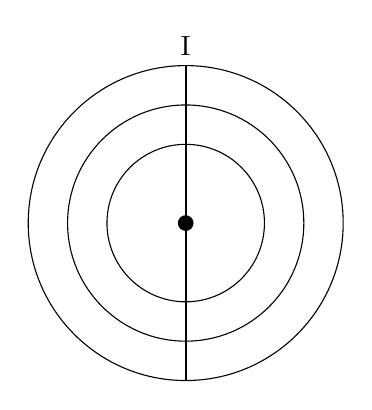
\begin{tikzpicture}
\draw[thick] (0,-2) -- (0,2);
\draw[->] (0,0) node[circle,fill,inner sep=2pt] {} circle (1);
\draw[->] (0,0) circle (1.5);
\draw[->] (0,0) circle (2);
\node[above] at (0,2) {I};
\end{tikzpicture}

a) State the direction of the magnetic field
b) How does field strength vary with distance?

\end{document}
